% Options for packages loaded elsewhere
\PassOptionsToPackage{unicode}{hyperref}
\PassOptionsToPackage{hyphens}{url}
%
\documentclass[
]{article}
\usepackage{amsmath,amssymb}
\usepackage{iftex}
\ifPDFTeX
  \usepackage[T1]{fontenc}
  \usepackage[utf8]{inputenc}
  \usepackage{textcomp} % provide euro and other symbols
\else % if luatex or xetex
  \usepackage{unicode-math} % this also loads fontspec
  \defaultfontfeatures{Scale=MatchLowercase}
  \defaultfontfeatures[\rmfamily]{Ligatures=TeX,Scale=1}
\fi
\usepackage{lmodern}
\ifPDFTeX\else
  % xetex/luatex font selection
\fi
% Use upquote if available, for straight quotes in verbatim environments
\IfFileExists{upquote.sty}{\usepackage{upquote}}{}
\IfFileExists{microtype.sty}{% use microtype if available
  \usepackage[]{microtype}
  \UseMicrotypeSet[protrusion]{basicmath} % disable protrusion for tt fonts
}{}
\makeatletter
\@ifundefined{KOMAClassName}{% if non-KOMA class
  \IfFileExists{parskip.sty}{%
    \usepackage{parskip}
  }{% else
    \setlength{\parindent}{0pt}
    \setlength{\parskip}{6pt plus 2pt minus 1pt}}
}{% if KOMA class
  \KOMAoptions{parskip=half}}
\makeatother
\usepackage{xcolor}
\usepackage[margin=1in]{geometry}
\usepackage{color}
\usepackage{fancyvrb}
\newcommand{\VerbBar}{|}
\newcommand{\VERB}{\Verb[commandchars=\\\{\}]}
\DefineVerbatimEnvironment{Highlighting}{Verbatim}{commandchars=\\\{\}}
% Add ',fontsize=\small' for more characters per line
\usepackage{framed}
\definecolor{shadecolor}{RGB}{248,248,248}
\newenvironment{Shaded}{\begin{snugshade}}{\end{snugshade}}
\newcommand{\AlertTok}[1]{\textcolor[rgb]{0.94,0.16,0.16}{#1}}
\newcommand{\AnnotationTok}[1]{\textcolor[rgb]{0.56,0.35,0.01}{\textbf{\textit{#1}}}}
\newcommand{\AttributeTok}[1]{\textcolor[rgb]{0.13,0.29,0.53}{#1}}
\newcommand{\BaseNTok}[1]{\textcolor[rgb]{0.00,0.00,0.81}{#1}}
\newcommand{\BuiltInTok}[1]{#1}
\newcommand{\CharTok}[1]{\textcolor[rgb]{0.31,0.60,0.02}{#1}}
\newcommand{\CommentTok}[1]{\textcolor[rgb]{0.56,0.35,0.01}{\textit{#1}}}
\newcommand{\CommentVarTok}[1]{\textcolor[rgb]{0.56,0.35,0.01}{\textbf{\textit{#1}}}}
\newcommand{\ConstantTok}[1]{\textcolor[rgb]{0.56,0.35,0.01}{#1}}
\newcommand{\ControlFlowTok}[1]{\textcolor[rgb]{0.13,0.29,0.53}{\textbf{#1}}}
\newcommand{\DataTypeTok}[1]{\textcolor[rgb]{0.13,0.29,0.53}{#1}}
\newcommand{\DecValTok}[1]{\textcolor[rgb]{0.00,0.00,0.81}{#1}}
\newcommand{\DocumentationTok}[1]{\textcolor[rgb]{0.56,0.35,0.01}{\textbf{\textit{#1}}}}
\newcommand{\ErrorTok}[1]{\textcolor[rgb]{0.64,0.00,0.00}{\textbf{#1}}}
\newcommand{\ExtensionTok}[1]{#1}
\newcommand{\FloatTok}[1]{\textcolor[rgb]{0.00,0.00,0.81}{#1}}
\newcommand{\FunctionTok}[1]{\textcolor[rgb]{0.13,0.29,0.53}{\textbf{#1}}}
\newcommand{\ImportTok}[1]{#1}
\newcommand{\InformationTok}[1]{\textcolor[rgb]{0.56,0.35,0.01}{\textbf{\textit{#1}}}}
\newcommand{\KeywordTok}[1]{\textcolor[rgb]{0.13,0.29,0.53}{\textbf{#1}}}
\newcommand{\NormalTok}[1]{#1}
\newcommand{\OperatorTok}[1]{\textcolor[rgb]{0.81,0.36,0.00}{\textbf{#1}}}
\newcommand{\OtherTok}[1]{\textcolor[rgb]{0.56,0.35,0.01}{#1}}
\newcommand{\PreprocessorTok}[1]{\textcolor[rgb]{0.56,0.35,0.01}{\textit{#1}}}
\newcommand{\RegionMarkerTok}[1]{#1}
\newcommand{\SpecialCharTok}[1]{\textcolor[rgb]{0.81,0.36,0.00}{\textbf{#1}}}
\newcommand{\SpecialStringTok}[1]{\textcolor[rgb]{0.31,0.60,0.02}{#1}}
\newcommand{\StringTok}[1]{\textcolor[rgb]{0.31,0.60,0.02}{#1}}
\newcommand{\VariableTok}[1]{\textcolor[rgb]{0.00,0.00,0.00}{#1}}
\newcommand{\VerbatimStringTok}[1]{\textcolor[rgb]{0.31,0.60,0.02}{#1}}
\newcommand{\WarningTok}[1]{\textcolor[rgb]{0.56,0.35,0.01}{\textbf{\textit{#1}}}}
\usepackage{graphicx}
\makeatletter
\def\maxwidth{\ifdim\Gin@nat@width>\linewidth\linewidth\else\Gin@nat@width\fi}
\def\maxheight{\ifdim\Gin@nat@height>\textheight\textheight\else\Gin@nat@height\fi}
\makeatother
% Scale images if necessary, so that they will not overflow the page
% margins by default, and it is still possible to overwrite the defaults
% using explicit options in \includegraphics[width, height, ...]{}
\setkeys{Gin}{width=\maxwidth,height=\maxheight,keepaspectratio}
% Set default figure placement to htbp
\makeatletter
\def\fps@figure{htbp}
\makeatother
\setlength{\emergencystretch}{3em} % prevent overfull lines
\providecommand{\tightlist}{%
  \setlength{\itemsep}{0pt}\setlength{\parskip}{0pt}}
\setcounter{secnumdepth}{5}
% Load necessary packages
\usepackage{amsmath}    % For advanced math typesetting
\usepackage{graphicx}   % For including images
\usepackage{hyperref}   % For hyperlinks
\usepackage{geometry}   % For setting page dimensions
\usepackage{fancyhdr}   % For custom headers and footers
\usepackage{setspace}   % For setting line spacing

% Set page dimensions
\geometry{
  a4paper,
  left=25mm,
  right=25mm,
  top=25mm,
  bottom=25mm
}

% Custom header and footer
\pagestyle{fancy}
\fancyhf{}
\fancyhead[L]{\leftmark}
\fancyhead[R]{\thepage}

% Custom commands
\newcommand{\HRule}{\rule{\linewidth}{0.5mm}}

% Set line spacing
\setstretch{1.5}

% Additional settings
\hypersetup{
  colorlinks=true,
  linkcolor=blue,
  filecolor=magenta,
  urlcolor=cyan,
  pdftitle={Your Document Title},
  pdfpagemode=FullScreen,
}
\ifLuaTeX
  \usepackage{selnolig}  % disable illegal ligatures
\fi
\IfFileExists{bookmark.sty}{\usepackage{bookmark}}{\usepackage{hyperref}}
\IfFileExists{xurl.sty}{\usepackage{xurl}}{} % add URL line breaks if available
\urlstyle{same}
\hypersetup{
  pdftitle={C91AR: Advanced Statistics using R},
  pdfauthor={Dr Peter E McKenna},
  hidelinks,
  pdfcreator={LaTeX via pandoc}}

\title{C91AR: Advanced Statistics using R}
\usepackage{etoolbox}
\makeatletter
\providecommand{\subtitle}[1]{% add subtitle to \maketitle
  \apptocmd{\@title}{\par {\large #1 \par}}{}{}
}
\makeatother
\subtitle{Wrangling Real Data}
\author{Dr Peter E McKenna}
\date{2025-02-11}

\begin{document}
\maketitle

{
\setcounter{tocdepth}{2}
\tableofcontents
}
\hypertarget{packages-for-todays-session}{%
\section{Packages for todays
session}\label{packages-for-todays-session}}

\begin{Shaded}
\begin{Highlighting}[]
\CommentTok{\# Load packages}
\NormalTok{pacman}\SpecialCharTok{::}\FunctionTok{p\_load}\NormalTok{(tidyverse,}
\NormalTok{               broom,}
\NormalTok{               GGally,}
\NormalTok{               nortest,}
\NormalTok{               psych)}
\end{Highlighting}
\end{Shaded}

\hypertarget{what-are-we-going-to-cover-today}{%
\section{What are we going to cover
today}\label{what-are-we-going-to-cover-today}}

\begin{itemize}
\tightlist
\item
  Wrangling, summarising, and visualising numeric data
\item
  Assessing the distribution of numeric data (though we will cover this
  more thoroughly in week 7)
\item
  Wrangling, summarising, and visualising categorical data
\end{itemize}

\hypertarget{summarising-data-in-r}{%
\section{Summarising data in R}\label{summarising-data-in-r}}

\begin{itemize}
\tightlist
\item
  Now that we've looked at how to keep code tidy and how to tidy our
  data, build on what we've started to learn from the data wrangling
  operations
\item
  I've shown you how to filter and select your data, and by adding more
  commands to your chain of pipes (\texttt{\textbar{}\textgreater{}})
  you can also start to generate summaries of your data
\end{itemize}

\hypertarget{using-pipes-to-generate-summaries}{%
\section{Using pipes to generate
summaries}\label{using-pipes-to-generate-summaries}}

\begin{itemize}
\tightlist
\item
  Think about your data and what summaries would be useful for your
  research
\item
  Let's read in our tidy data to get started
\end{itemize}

\begin{Shaded}
\begin{Highlighting}[]
\CommentTok{\# Read in the tidy data}
\NormalTok{df }\OtherTok{\textless{}{-}}
  \FunctionTok{read\_csv}\NormalTok{(}\StringTok{"data\_tidy/c91ar\_maze\_data.csv"}\NormalTok{,}
           \AttributeTok{col\_types =} \StringTok{"cccdccd"}\NormalTok{) }\SpecialCharTok{|\textgreater{}}
  \FunctionTok{drop\_na}\NormalTok{()}\CommentTok{\# omit NAs}
\end{Highlighting}
\end{Shaded}

\hypertarget{examine-the-data}{%
\section{Examine the data}\label{examine-the-data}}

\begin{Shaded}
\begin{Highlighting}[]
\CommentTok{\# Examine the data}
\FunctionTok{glimpse}\NormalTok{(df)}
\end{Highlighting}
\end{Shaded}

\hypertarget{dataset-metadata}{%
\section{Dataset Metadata}\label{dataset-metadata}}

\begin{itemize}
\tightlist
\item
  \texttt{id} = anon participant code
\item
  \texttt{condition} = ToM manipulation with three levels (Baseline,
  No-ToM, and ToM)
\item
  \texttt{trial} = experiment trial
\item
  \texttt{rt} = response time
\item
  \texttt{follow\ robot} = whether participants followed the robot's
  suggestion
\item
  \texttt{accuracy} = whether or not their maze route selection was
  correct
\item
  \texttt{conf} = participants self reported confidence for each route
  decision.
\end{itemize}

\hypertarget{reseach-questions}{%
\section{Reseach questions}\label{reseach-questions}}

\begin{itemize}
\tightlist
\item
  Did robot ToM affect participants trust?
\item
  Did robot ToM affect participants task performance?

  \begin{itemize}
  \tightlist
  \item
    Decision time
  \item
    Confidence
  \end{itemize}
\end{itemize}

\hypertarget{descriptive-statistics}{%
\section{Descriptive Statistics}\label{descriptive-statistics}}

\begin{itemize}
\tightlist
\item
  We use a combination of \emph{Tidyverse} verbs to select, group and
  summarise data

  \begin{itemize}
  \tightlist
  \item
    \texttt{group\_by}
  \item
    \texttt{select}
  \item
    \texttt{arrange}
  \item
    \texttt{filter}
  \item
    \texttt{summarise}
  \end{itemize}
\end{itemize}

\begin{center}\rule{0.5\linewidth}{0.5pt}\end{center}

\begin{Shaded}
\begin{Highlighting}[]
\NormalTok{df }\SpecialCharTok{|\textgreater{}}
  \FunctionTok{select}\NormalTok{(rt,}
\NormalTok{         conf) }\SpecialCharTok{|\textgreater{}}
  \FunctionTok{ggpairs}\NormalTok{() }\CommentTok{\# from GGally}
\end{Highlighting}
\end{Shaded}

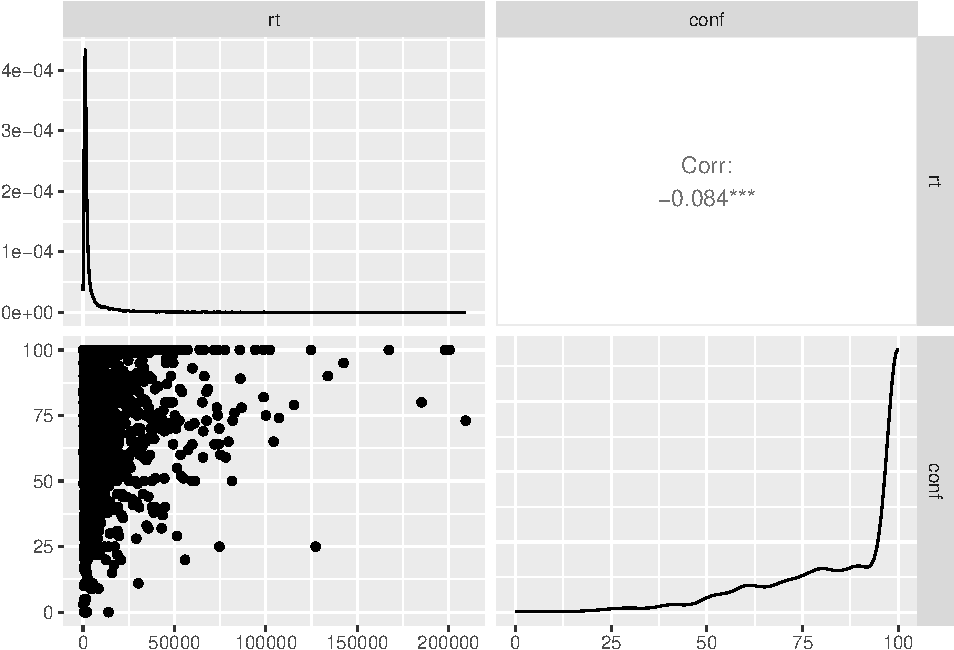
\includegraphics{T5_Data_wrangling_pdf_files/figure-latex/unnamed-chunk-5-1.pdf}

\begin{center}\rule{0.5\linewidth}{0.5pt}\end{center}

\begin{itemize}
\tightlist
\item
  You can see that \texttt{rt} is positively skewed and \texttt{conf} is
  negatively skewed
\item
  Think, \textbf{where is the tail?}
\end{itemize}

\begin{Shaded}
\begin{Highlighting}[]
\CommentTok{\# Test the normality of rt}
\CommentTok{\# shapiro.test(df$rt) }


\CommentTok{\# Test the normlisaty of conf}
\CommentTok{\# shapiro.test(df$conf)}


\CommentTok{\# For large datasets, use Anderson{-}Darling instead}
  \CommentTok{\# Null hypothesis is that the data follows a particular distribution}
\CommentTok{\#library(nortest)}

\CommentTok{\# response time}
\FunctionTok{ad.test}\NormalTok{(df}\SpecialCharTok{$}\NormalTok{rt)}

\CommentTok{\# confidence}
\FunctionTok{ad.test}\NormalTok{(df}\SpecialCharTok{$}\NormalTok{conf)}
\end{Highlighting}
\end{Shaded}

\begin{itemize}
\tightlist
\item
  So, both \texttt{rt} and \texttt{conf} are not normally distributed
\end{itemize}

\hypertarget{working-with-reactiondecision-time-data}{%
\section{Working with reaction/decision time
data}\label{working-with-reactiondecision-time-data}}

\begin{itemize}
\tightlist
\item
  Sometimes, you have to make a judgement call about what constitutes a
  theoretically valid response in your experiment.
\item
  The minimum RT here is below zero, which is not possible
\item
  One way to make an educated guess is to examine the histogram and hone
  in on the region of interest
\item
  But, before I go any further\ldots{}
\end{itemize}

\hypertarget{data-visualisation-with-ggplot2}{%
\section{\texorpdfstring{Data Visualisation with
\texttt{ggplot2}}{Data Visualisation with ggplot2}}\label{data-visualisation-with-ggplot2}}

\begin{itemize}
\tightlist
\item
  This is the package used to produce plots in R
\item
  It comes with a whole host of its own functions and is very flexible
  in terms of the graphical aesthetics.
\item
  Annoyingly, it does not use \texttt{\textbar{}\textgreater{}} (e.g.,
  pipes) but instead uses the \texttt{+} symbol.
\item
  So, when you combine \emph{Tidyverse} and \emph{ggplot2} you often see
  a combination beginning with \texttt{\textbar{}\textgreater{}} and
  ending with \texttt{+} to chain commands together.
\end{itemize}

\hypertarget{visualising-distributions-using-ggplot2}{%
\section{\texorpdfstring{Visualising distributions using
\texttt{ggplot2}}{Visualising distributions using ggplot2}}\label{visualising-distributions-using-ggplot2}}

\begin{Shaded}
\begin{Highlighting}[]
\CommentTok{\# Visualise the full rt distribution}
\NormalTok{df }\SpecialCharTok{|\textgreater{}}
  \FunctionTok{select}\NormalTok{(rt) }\SpecialCharTok{|\textgreater{}}
  \FunctionTok{ggplot}\NormalTok{(}\AttributeTok{mapping =} \FunctionTok{aes}\NormalTok{(rt)) }\SpecialCharTok{+}
  \FunctionTok{geom\_histogram}\NormalTok{(}\AttributeTok{bins =} \DecValTok{100}\NormalTok{) }\SpecialCharTok{+} 
  \FunctionTok{labs}\NormalTok{(}\AttributeTok{y =} \StringTok{"Frequency"}\NormalTok{,}
       \AttributeTok{title =} \StringTok{"Histogram of Response time (ms) distribution"}\NormalTok{)}
\end{Highlighting}
\end{Shaded}

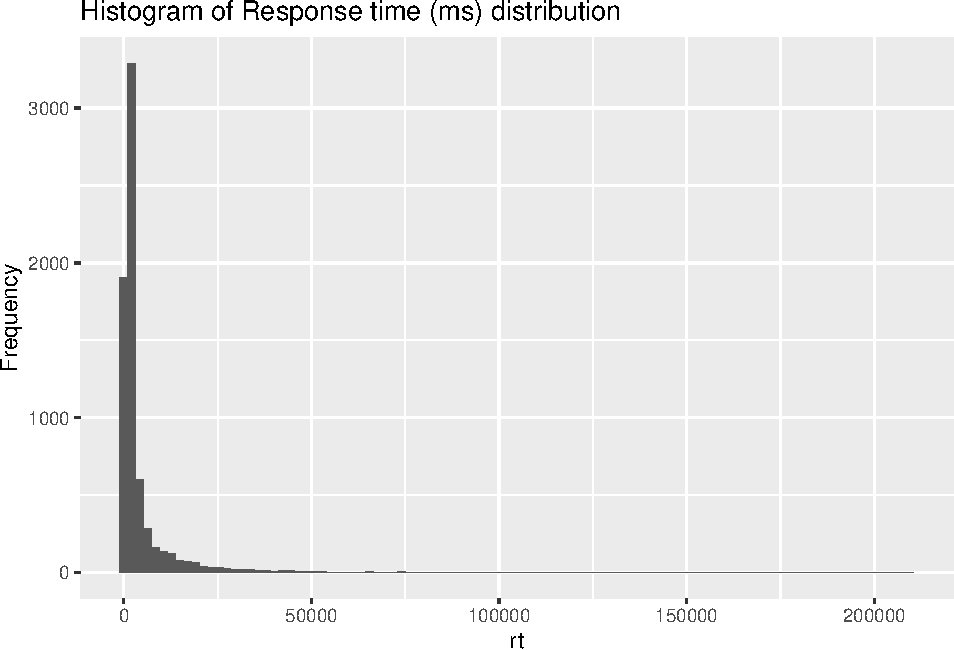
\includegraphics{T5_Data_wrangling_pdf_files/figure-latex/unnamed-chunk-7-1.pdf}

\begin{center}\rule{0.5\linewidth}{0.5pt}\end{center}

\begin{Shaded}
\begin{Highlighting}[]
\CommentTok{\# Visualise the full conf distribution}
\NormalTok{df }\SpecialCharTok{|\textgreater{}}
  \FunctionTok{select}\NormalTok{(conf) }\SpecialCharTok{|\textgreater{}}
  \FunctionTok{ggplot}\NormalTok{(}\AttributeTok{mapping =} \FunctionTok{aes}\NormalTok{(conf)) }\SpecialCharTok{+}
  \FunctionTok{geom\_histogram}\NormalTok{(}\AttributeTok{bins =} \DecValTok{30}\NormalTok{) }\SpecialCharTok{+} 
  \FunctionTok{labs}\NormalTok{(}\AttributeTok{y =} \StringTok{"Frequency"}\NormalTok{,}
       \AttributeTok{title =} \StringTok{"Histogram of Response time (ms) distribution"}\NormalTok{)}
\end{Highlighting}
\end{Shaded}

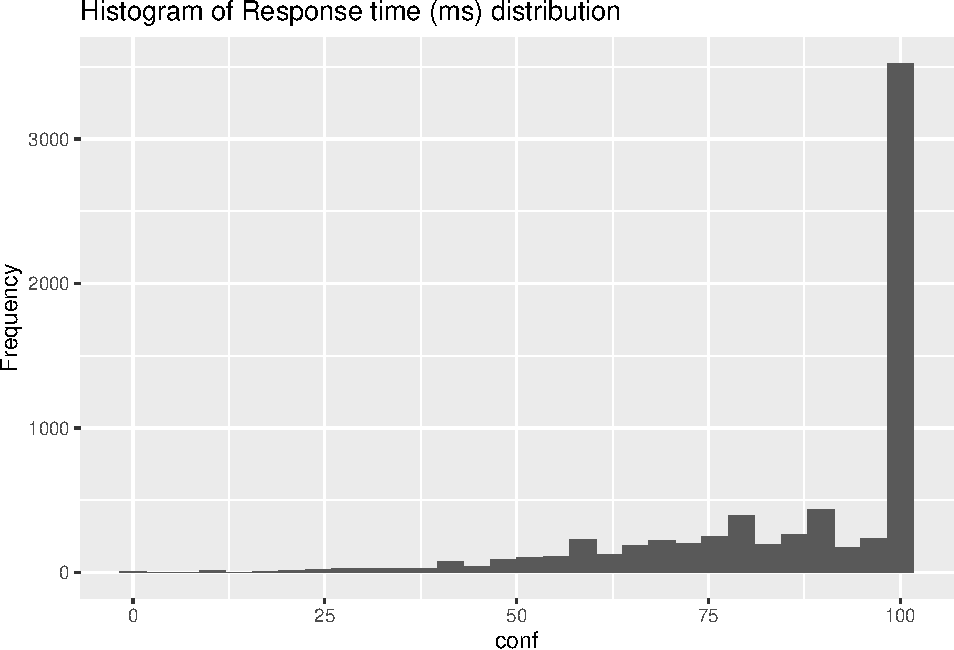
\includegraphics{T5_Data_wrangling_pdf_files/figure-latex/unnamed-chunk-8-1.pdf}

\hypertarget{taking-a-closer-look-at-the-distribution-extremities}{%
\section{Taking a closer look at the distribution
extremities}\label{taking-a-closer-look-at-the-distribution-extremities}}

\begin{Shaded}
\begin{Highlighting}[]
\CommentTok{\# Visualise the observations near the y{-}axis origin}
\NormalTok{df }\SpecialCharTok{|\textgreater{}}
  \FunctionTok{filter}\NormalTok{(rt }\SpecialCharTok{\%in\%} \FunctionTok{c}\NormalTok{(}\DecValTok{0}\SpecialCharTok{:}\DecValTok{700}\NormalTok{)) }\SpecialCharTok{|\textgreater{}} \CommentTok{\# I\textquotesingle{}m not interested in values below zero}
  \FunctionTok{ggplot}\NormalTok{(}\AttributeTok{mapping =} \FunctionTok{aes}\NormalTok{(rt)) }\SpecialCharTok{+}
  \FunctionTok{geom\_histogram}\NormalTok{(}\AttributeTok{bins =} \DecValTok{30}\NormalTok{) }\SpecialCharTok{+} 
  \FunctionTok{labs}\NormalTok{(}\AttributeTok{y =} \StringTok{"Frequency"}\NormalTok{,}
       \AttributeTok{title =} \StringTok{"Histogram of Response time (ms) distribution"}\NormalTok{)}
\end{Highlighting}
\end{Shaded}

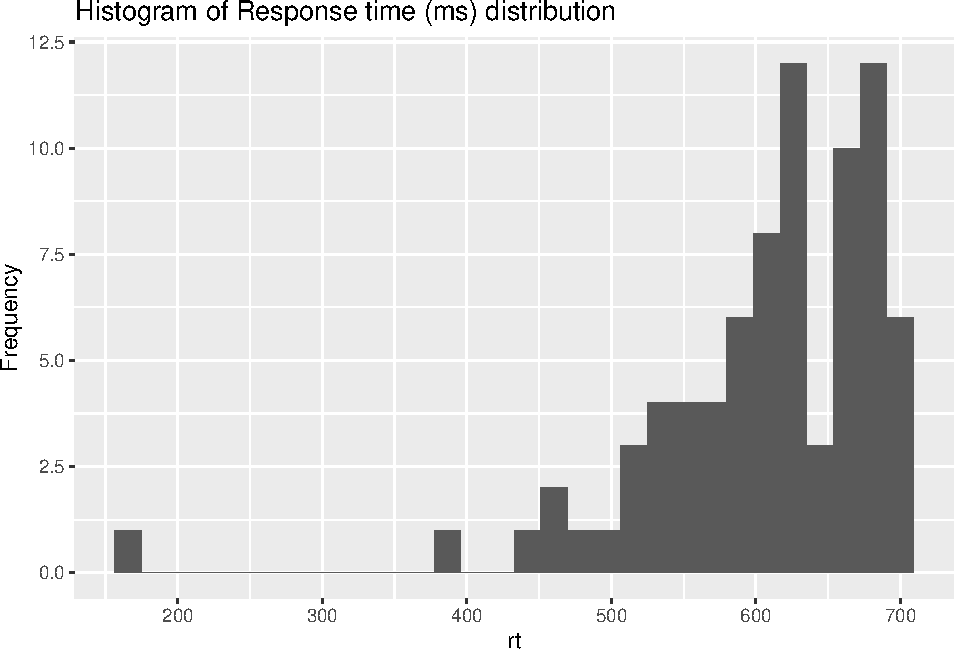
\includegraphics{T5_Data_wrangling_pdf_files/figure-latex/unnamed-chunk-9-1.pdf}

\begin{center}\rule{0.5\linewidth}{0.5pt}\end{center}

\begin{Shaded}
\begin{Highlighting}[]
\CommentTok{\# Visualise the observations at the tail of the distribution}
\NormalTok{df }\SpecialCharTok{|\textgreater{}}
  \FunctionTok{filter}\NormalTok{(rt }\SpecialCharTok{\%in\%} \FunctionTok{c}\NormalTok{(}\DecValTok{1500}\SpecialCharTok{:}\DecValTok{6000}\NormalTok{)) }\SpecialCharTok{|\textgreater{}}
  \FunctionTok{ggplot}\NormalTok{(}\AttributeTok{mapping =} \FunctionTok{aes}\NormalTok{(rt)) }\SpecialCharTok{+}
  \FunctionTok{geom\_histogram}\NormalTok{(}\AttributeTok{bins =} \DecValTok{30}\NormalTok{) }\SpecialCharTok{+} 
  \FunctionTok{labs}\NormalTok{(}\AttributeTok{y =} \StringTok{"Frequency"}\NormalTok{,}
       \AttributeTok{title =} \StringTok{"Histogram of Response time (ms) distribution"}\NormalTok{)}
\end{Highlighting}
\end{Shaded}

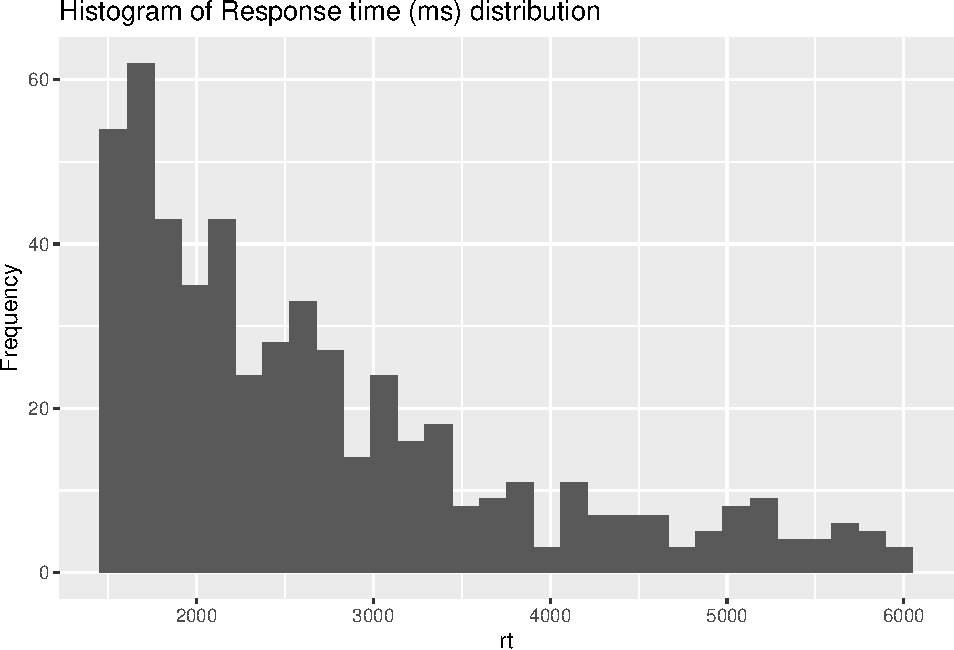
\includegraphics{T5_Data_wrangling_pdf_files/figure-latex/unnamed-chunk-10-1.pdf}

\hypertarget{based-on-the-following-plot-where-would-say-is-safe-to-start-our-distribution}{%
\section{Based on the following plot, where would say is safe to start
our
distribution?}\label{based-on-the-following-plot-where-would-say-is-safe-to-start-our-distribution}}

\hypertarget{visualise-new-distribution}{%
\section{Visualise new distribution}\label{visualise-new-distribution}}

\begin{Shaded}
\begin{Highlighting}[]
\CommentTok{\# Visualise the observations included in our new limits}
\NormalTok{df }\SpecialCharTok{|\textgreater{}}
  \FunctionTok{filter}\NormalTok{(rt }\SpecialCharTok{\%in\%} \FunctionTok{c}\NormalTok{(}\DecValTok{500}\SpecialCharTok{:}\DecValTok{5000}\NormalTok{)) }\SpecialCharTok{|\textgreater{}}
  \FunctionTok{ggplot}\NormalTok{(}\AttributeTok{mapping =} \FunctionTok{aes}\NormalTok{(rt)) }\SpecialCharTok{+}
  \FunctionTok{geom\_histogram}\NormalTok{(}\AttributeTok{bins =} \DecValTok{30}\NormalTok{) }\SpecialCharTok{+} 
  \FunctionTok{labs}\NormalTok{(}\AttributeTok{y =} \StringTok{"Frequency"}\NormalTok{,}
       \AttributeTok{title =} \StringTok{"Histogram of Response time (ms) distribution"}\NormalTok{)}
\end{Highlighting}
\end{Shaded}

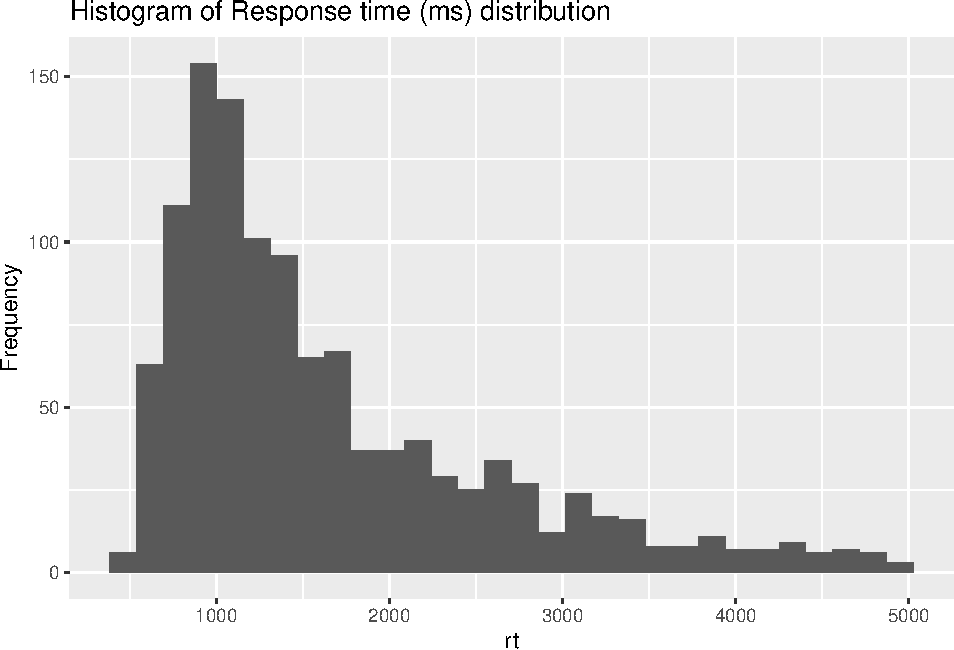
\includegraphics{T5_Data_wrangling_pdf_files/figure-latex/unnamed-chunk-11-1.pdf}

\hypertarget{visualise-transformed-data}{%
\section{Visualise transformed data}\label{visualise-transformed-data}}

\begin{itemize}
\tightlist
\item
  This measure is one approach to normalise positively and negatively
  skewed distributions
\end{itemize}

\begin{Shaded}
\begin{Highlighting}[]
\CommentTok{\# Visualise the log transformed rt}
\NormalTok{df }\SpecialCharTok{|\textgreater{}}
\NormalTok{  dplyr}\SpecialCharTok{::}\FunctionTok{filter}\NormalTok{(rt }\SpecialCharTok{\%in\%} \FunctionTok{c}\NormalTok{(}\DecValTok{500}\SpecialCharTok{:}\DecValTok{5000}\NormalTok{)) }\SpecialCharTok{|\textgreater{}}
  \FunctionTok{ggplot}\NormalTok{(}\AttributeTok{mapping =} \FunctionTok{aes}\NormalTok{(}\FunctionTok{log}\NormalTok{(rt))) }\SpecialCharTok{+}
  \FunctionTok{geom\_histogram}\NormalTok{(}\AttributeTok{bins =} \DecValTok{30}\NormalTok{) }\SpecialCharTok{+} 
  \FunctionTok{labs}\NormalTok{(}\AttributeTok{y =} \StringTok{"Frequency"}\NormalTok{,}
       \AttributeTok{title =} \StringTok{"Histogram of log(response time; ms) distribution"}\NormalTok{)}
\end{Highlighting}
\end{Shaded}

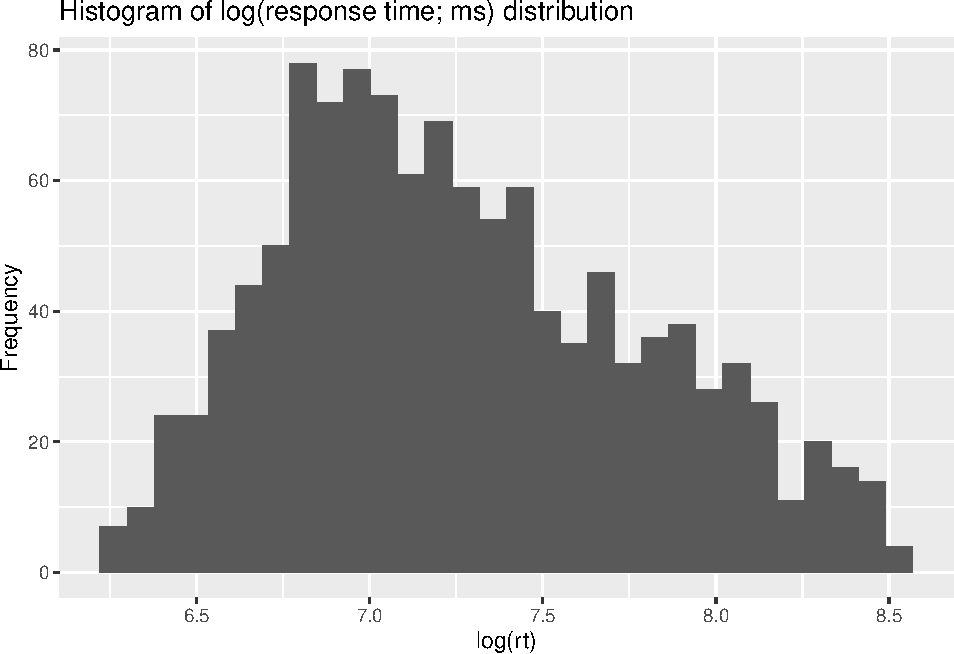
\includegraphics{T5_Data_wrangling_pdf_files/figure-latex/unnamed-chunk-12-1.pdf}

\begin{center}\rule{0.5\linewidth}{0.5pt}\end{center}

\begin{Shaded}
\begin{Highlighting}[]
\CommentTok{\# Visualise the log transformed conf}
\NormalTok{df }\SpecialCharTok{|\textgreater{}}
  \FunctionTok{filter}\NormalTok{(rt }\SpecialCharTok{\%in\%} \FunctionTok{c}\NormalTok{(}\DecValTok{500}\SpecialCharTok{:}\DecValTok{5000}\NormalTok{)) }\SpecialCharTok{|\textgreater{}}
  \FunctionTok{ggplot}\NormalTok{(}\AttributeTok{mapping =} \FunctionTok{aes}\NormalTok{(}\FunctionTok{log}\NormalTok{(conf))) }\SpecialCharTok{+}
  \FunctionTok{geom\_histogram}\NormalTok{(}\AttributeTok{bins =} \DecValTok{30}\NormalTok{) }\SpecialCharTok{+} 
  \FunctionTok{labs}\NormalTok{(}\AttributeTok{y =} \StringTok{"Frequency"}\NormalTok{,}
       \AttributeTok{title =} \StringTok{"Histogram of log(confidence) distribution"}\NormalTok{)}
\end{Highlighting}
\end{Shaded}

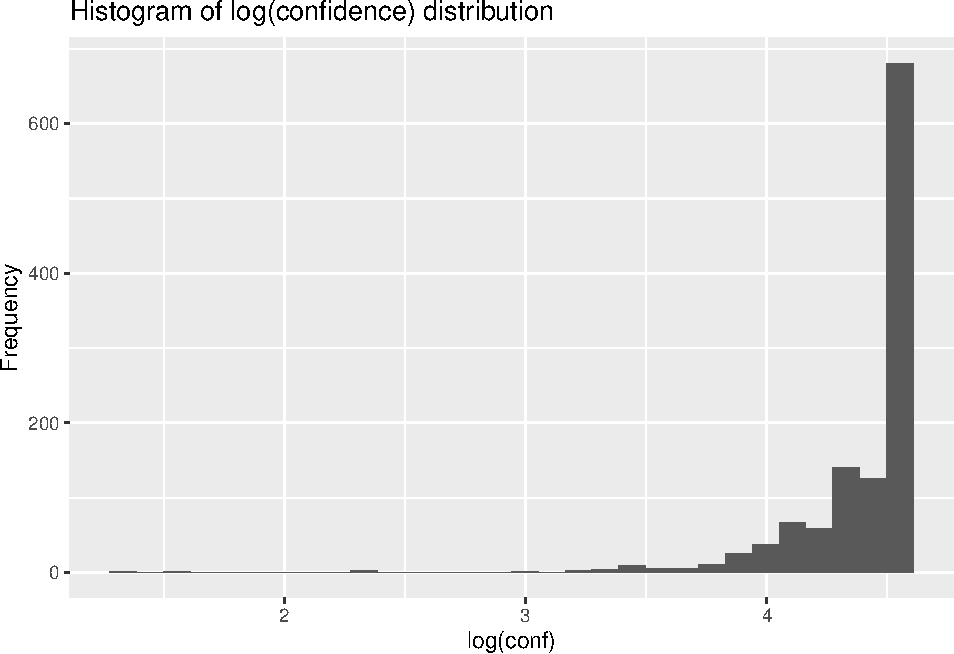
\includegraphics{T5_Data_wrangling_pdf_files/figure-latex/unnamed-chunk-13-1.pdf}

\hypertarget{checking-correlations-based-on-new-parameters}{%
\section{Checking correlations based on new
parameters}\label{checking-correlations-based-on-new-parameters}}

\begin{Shaded}
\begin{Highlighting}[]
\NormalTok{df }\SpecialCharTok{|\textgreater{}}
  \FunctionTok{filter}\NormalTok{(rt }\SpecialCharTok{\%in\%} \FunctionTok{c}\NormalTok{(}\DecValTok{500}\SpecialCharTok{:}\DecValTok{3000}\NormalTok{)) }\SpecialCharTok{|\textgreater{}} \CommentTok{\# filter the data}
  \FunctionTok{mutate}\NormalTok{(}\AttributeTok{rt\_log =} \FunctionTok{log}\NormalTok{(rt),}
         \AttributeTok{conf\_log =} \FunctionTok{log}\NormalTok{(conf)) }\SpecialCharTok{|\textgreater{}} \CommentTok{\# create a log of rt vector }
  \FunctionTok{select}\NormalTok{(rt\_log,}
\NormalTok{         conf\_log) }\SpecialCharTok{|\textgreater{}} \CommentTok{\# only include numeric vectors}
  \FunctionTok{ggpairs}\NormalTok{()}
\end{Highlighting}
\end{Shaded}

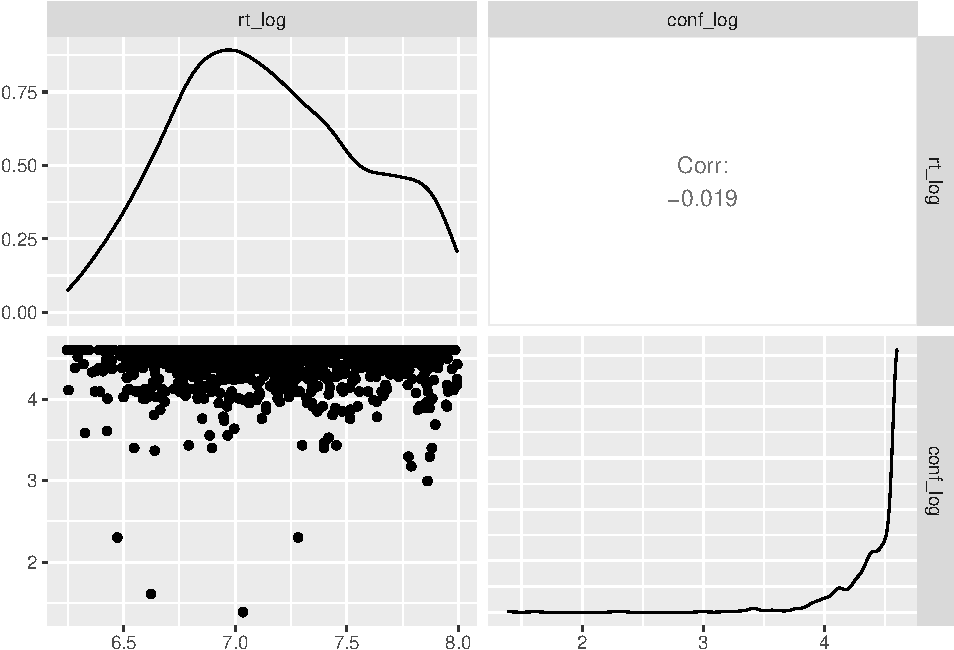
\includegraphics{T5_Data_wrangling_pdf_files/figure-latex/unnamed-chunk-14-1.pdf}

\begin{itemize}
\tightlist
\item
  According to our new limits and log transformation, there is no
  correlation between response time and confidence.
\end{itemize}

\hypertarget{tom-condition-descrtiptives}{%
\section{ToM condition
descrtiptives}\label{tom-condition-descrtiptives}}

\begin{Shaded}
\begin{Highlighting}[]
\CommentTok{\# create a new object based on our chosen rt parameters}

\NormalTok{df1 }\OtherTok{\textless{}{-}}
\NormalTok{  df }\SpecialCharTok{|\textgreater{}}
  \FunctionTok{filter}\NormalTok{(rt }\SpecialCharTok{\%in\%} \FunctionTok{c}\NormalTok{(}\DecValTok{500}\SpecialCharTok{:}\DecValTok{5000}\NormalTok{)) }\SpecialCharTok{|\textgreater{}}
  \FunctionTok{mutate}\NormalTok{(}\AttributeTok{rt\_log =} \FunctionTok{log}\NormalTok{(rt),}
         \AttributeTok{conf\_log =} \FunctionTok{log}\NormalTok{(conf)) }\SpecialCharTok{|\textgreater{}}
  \FunctionTok{mutate\_if}\NormalTok{(is.character, as.factor)}
\end{Highlighting}
\end{Shaded}

\hypertarget{creating-new-tibblesobjects}{%
\section{Creating new
tibbles/objects}\label{creating-new-tibblesobjects}}

\begin{itemize}
\tightlist
\item
  Be sure to create a comment explicitly stating what df1 represents
\item
  You could do this in a separate .txt file or in your script
\item
  The last line of the chain tells R to treat the character cols as
  factor, because converting factors back to characters is the default
  behaviour when creating new data objects
\item
  df1 = data with rt 500:5000
\end{itemize}

\begin{center}\rule{0.5\linewidth}{0.5pt}\end{center}

\begin{Shaded}
\begin{Highlighting}[]
\CommentTok{\# Summarise the data}
\NormalTok{df1 }\SpecialCharTok{|\textgreater{}}
  \FunctionTok{select}\NormalTok{(condition, }
\NormalTok{         rt\_log, }
\NormalTok{         conf\_log) }\SpecialCharTok{\%\textgreater{}\%}
  \FunctionTok{group\_by}\NormalTok{(condition) }\SpecialCharTok{\%\textgreater{}\%} 
  \FunctionTok{summarise}\NormalTok{(}\AttributeTok{avg\_rt =} \FunctionTok{mean}\NormalTok{(rt\_log), }\CommentTok{\# remember, we are operating in the log space now}
            \AttributeTok{sd\_rt =} \FunctionTok{sd}\NormalTok{(rt\_log),}
            \AttributeTok{med\_rt =} \FunctionTok{median}\NormalTok{(rt\_log),}
            \AttributeTok{avg\_conf =} \FunctionTok{mean}\NormalTok{(conf\_log),}
            \AttributeTok{sd\_conf =} \FunctionTok{sd}\NormalTok{(conf\_log),}
            \AttributeTok{med\_conf =} \FunctionTok{median}\NormalTok{(conf\_log))}
\end{Highlighting}
\end{Shaded}

\begin{verbatim}
## # A tibble: 3 x 7
##   condition avg_rt sd_rt med_rt avg_conf sd_conf med_conf
##   <fct>      <dbl> <dbl>  <dbl>    <dbl>   <dbl>    <dbl>
## 1 baseline    7.18 0.523   7.06     4.38   0.346     4.49
## 2 No-ToM      7.32 0.512   7.27     4.45   0.289     4.61
## 3 ToM         7.34 0.499   7.27     4.46   0.224     4.60
\end{verbatim}

\hypertarget{describing-numeric-vectors-using-psych-package}{%
\section{\texorpdfstring{Describing numeric vectors using \texttt{psych}
package}{Describing numeric vectors using psych package}}\label{describing-numeric-vectors-using-psych-package}}

\begin{Shaded}
\begin{Highlighting}[]
\CommentTok{\# Overall summary of rt}
\NormalTok{df1 }\SpecialCharTok{|\textgreater{}}
  \FunctionTok{describe}\NormalTok{(}\AttributeTok{omit =} \ConstantTok{TRUE}\NormalTok{) }\CommentTok{\# omit non{-}numeric vectors}
\end{Highlighting}
\end{Shaded}

\hypertarget{descritives-of-your-numeric-variables-per-each-level-of-the-predictors}{%
\section{Descritives of your numeric variables per each level of the
predictors}\label{descritives-of-your-numeric-variables-per-each-level-of-the-predictors}}

\begin{Shaded}
\begin{Highlighting}[]
\CommentTok{\# Condition level summary of rt}
\FunctionTok{describe}\NormalTok{(rt\_log }\SpecialCharTok{\textasciitilde{}}\NormalTok{ condition, }\AttributeTok{data=}\NormalTok{df1) }\CommentTok{\# remember, tilde means modelled by}
\end{Highlighting}
\end{Shaded}

\hypertarget{exercise-use-the-describe-function-from-the-psych-package-to-summarise-both-overall-and-group-trends-from-the-confidence-rating-participants-gave-after-each-decision.}{%
\section{\texorpdfstring{Exercise: use the \texttt{describe} function
from the \emph{psych} package to summarise both overall and group trends
from the confidence rating participants gave after each
decision.}{Exercise: use the describe function from the psych package to summarise both overall and group trends from the confidence rating participants gave after each decision.}}\label{exercise-use-the-describe-function-from-the-psych-package-to-summarise-both-overall-and-group-trends-from-the-confidence-rating-participants-gave-after-each-decision.}}

\hypertarget{summarising-the-categorical-variables}{%
\section{Summarising the categorical
variables}\label{summarising-the-categorical-variables}}

\begin{itemize}
\tightlist
\item
  In the long data format (which is the go-to for R) each row represents
  a unique observation in the data.
\item
  So, when you summarise categorical data, you need to input the number
  of rows into the calculation to compute overall proportions.
\end{itemize}

\begin{Shaded}
\begin{Highlighting}[]
\CommentTok{\# How often did participants in each group follow the robots advice?}
\NormalTok{total\_n }\OtherTok{\textless{}{-}} 
  \FunctionTok{nrow}\NormalTok{(df1) }\CommentTok{\# nrow counts the number of rows}

\NormalTok{df1 }\SpecialCharTok{|\textgreater{}}
  \FunctionTok{group\_by}\NormalTok{(condition, follow\_robot) }\SpecialCharTok{|\textgreater{}}
  \FunctionTok{summarise}\NormalTok{(}\AttributeTok{n =} \FunctionTok{n}\NormalTok{(), }
            \AttributeTok{.groups =} \StringTok{\textquotesingle{}drop\textquotesingle{}}\NormalTok{) }\SpecialCharTok{|\textgreater{}} \CommentTok{\# ensures that the grouping is dropped after summarising}
  \FunctionTok{mutate}\NormalTok{(}\AttributeTok{freq =}\NormalTok{ n }\SpecialCharTok{/}\NormalTok{ total\_n) }\SpecialCharTok{|\textgreater{}}
  \FunctionTok{mutate}\NormalTok{(}\AttributeTok{freq =} \FunctionTok{round}\NormalTok{(freq }\SpecialCharTok{*} \DecValTok{100}\NormalTok{, }\AttributeTok{digits =} \DecValTok{2}\NormalTok{))}
\end{Highlighting}
\end{Shaded}

\hypertarget{visualising-categorical-data-trends}{%
\section{Visualising categorical data
trends}\label{visualising-categorical-data-trends}}

\begin{Shaded}
\begin{Highlighting}[]
\NormalTok{p\_follow }\OtherTok{\textless{}{-}}
\NormalTok{  df1 }\SpecialCharTok{|\textgreater{}}
  \FunctionTok{group\_by}\NormalTok{(condition, follow\_robot) }\SpecialCharTok{|\textgreater{}}
  \FunctionTok{summarise}\NormalTok{(}\AttributeTok{n =} \FunctionTok{n}\NormalTok{(), }
            \AttributeTok{.groups =} \StringTok{\textquotesingle{}drop\textquotesingle{}}\NormalTok{) }\SpecialCharTok{|\textgreater{}} \CommentTok{\# ensures that the grouping is dropped after summarising}
  \FunctionTok{mutate}\NormalTok{(}\AttributeTok{freq =}\NormalTok{ n }\SpecialCharTok{/}\NormalTok{ total\_n) }\SpecialCharTok{|\textgreater{}}
  \FunctionTok{mutate}\NormalTok{(}\AttributeTok{freq =} \FunctionTok{round}\NormalTok{(freq }\SpecialCharTok{*} \DecValTok{100}\NormalTok{, }\AttributeTok{digits =} \DecValTok{2}\NormalTok{))}

\NormalTok{p\_follow }\SpecialCharTok{|\textgreater{}}  
  \FunctionTok{ggplot}\NormalTok{(}\FunctionTok{aes}\NormalTok{(}\AttributeTok{x =}\NormalTok{ follow\_robot,}
                \AttributeTok{y =}\NormalTok{ freq,}
                \AttributeTok{fill =}\NormalTok{ condition,}
                \AttributeTok{group =}\NormalTok{ condition)) }\SpecialCharTok{+} 
  \FunctionTok{geom\_col}\NormalTok{(}\AttributeTok{stat =} \StringTok{"identity"}\NormalTok{,}
           \AttributeTok{position =} \StringTok{"dodge"}\NormalTok{) }\SpecialCharTok{+}
  \FunctionTok{labs}\NormalTok{(}\AttributeTok{title =} \StringTok{"Proportion of Robot Compliance per Condition"}\NormalTok{,}
       \AttributeTok{x =} \StringTok{"Compliance with Robot Route Advice"}\NormalTok{,}
       \AttributeTok{y =} \StringTok{"Proportion of Responses (\%)"}\NormalTok{) }\SpecialCharTok{+}
  \FunctionTok{theme\_minimal}\NormalTok{()}
\end{Highlighting}
\end{Shaded}

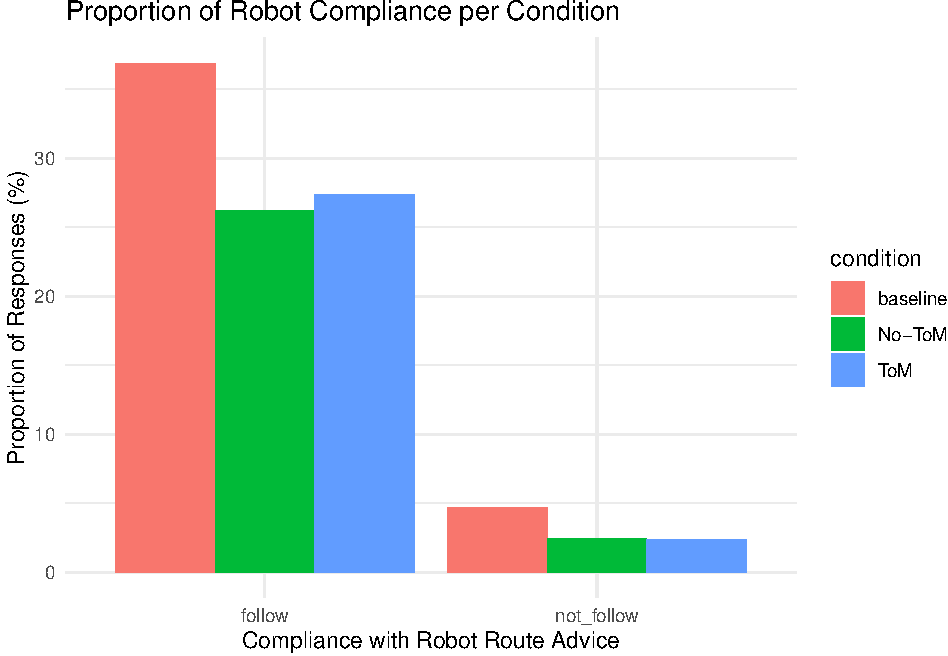
\includegraphics{T5_Data_wrangling_pdf_files/figure-latex/unnamed-chunk-20-1.pdf}

\begin{center}\rule{0.5\linewidth}{0.5pt}\end{center}

\begin{Shaded}
\begin{Highlighting}[]
\CommentTok{\# How often were participants correct in their route selection?}

\NormalTok{df1 }\SpecialCharTok{|\textgreater{}}
  \FunctionTok{group\_by}\NormalTok{(condition, }
\NormalTok{           accuracy) }\SpecialCharTok{|\textgreater{}}
  \FunctionTok{summarise}\NormalTok{(}\AttributeTok{n =} \FunctionTok{n}\NormalTok{(), }
            \AttributeTok{.groups =} \StringTok{\textquotesingle{}drop\textquotesingle{}}\NormalTok{) }\SpecialCharTok{|\textgreater{}} 
  \FunctionTok{mutate}\NormalTok{(}\AttributeTok{freq =}\NormalTok{ n }\SpecialCharTok{/}\NormalTok{ total\_n) }\SpecialCharTok{|\textgreater{}}
  \FunctionTok{mutate}\NormalTok{(}\AttributeTok{freq =} \FunctionTok{round}\NormalTok{(freq }\SpecialCharTok{*} \DecValTok{100}\NormalTok{, }\AttributeTok{digits =} \DecValTok{2}\NormalTok{))}
\end{Highlighting}
\end{Shaded}

\begin{verbatim}
## # A tibble: 6 x 4
##   condition accuracy      n  freq
##   <fct>     <fct>     <int> <dbl>
## 1 baseline  correct     402 34.2 
## 2 baseline  incorrect    87  7.4 
## 3 No-ToM    correct     308 26.2 
## 4 No-ToM    incorrect    29  2.47
## 5 ToM       correct     322 27.4 
## 6 ToM       incorrect    28  2.38
\end{verbatim}

\begin{center}\rule{0.5\linewidth}{0.5pt}\end{center}

\begin{Shaded}
\begin{Highlighting}[]
\NormalTok{p\_acc }\OtherTok{\textless{}{-}}
\NormalTok{  df1 }\SpecialCharTok{|\textgreater{}}
  \FunctionTok{group\_by}\NormalTok{(condition, }
\NormalTok{           accuracy) }\SpecialCharTok{|\textgreater{}}
  \FunctionTok{summarise}\NormalTok{(}\AttributeTok{n =} \FunctionTok{n}\NormalTok{(), }
            \AttributeTok{.groups =} \StringTok{\textquotesingle{}drop\textquotesingle{}}\NormalTok{) }\SpecialCharTok{|\textgreater{}} 
  \FunctionTok{mutate}\NormalTok{(}\AttributeTok{freq =}\NormalTok{ n }\SpecialCharTok{/}\NormalTok{ total\_n) }\SpecialCharTok{|\textgreater{}}
  \FunctionTok{mutate}\NormalTok{(}\AttributeTok{freq =} \FunctionTok{round}\NormalTok{(freq }\SpecialCharTok{*} \DecValTok{100}\NormalTok{, }\AttributeTok{digits =} \DecValTok{2}\NormalTok{))}

\NormalTok{p\_acc }\SpecialCharTok{|\textgreater{}}  
  \FunctionTok{ggplot}\NormalTok{(}\FunctionTok{aes}\NormalTok{(}\AttributeTok{x =}\NormalTok{ accuracy,}
                \AttributeTok{y =}\NormalTok{ freq,}
                \AttributeTok{fill =}\NormalTok{ condition,}
                \AttributeTok{group =}\NormalTok{ condition)) }\SpecialCharTok{+} 
  \FunctionTok{geom\_col}\NormalTok{(}\AttributeTok{stat =} \StringTok{"identity"}\NormalTok{,}
           \AttributeTok{position =} \StringTok{"dodge"}\NormalTok{) }\SpecialCharTok{+}
  \FunctionTok{labs}\NormalTok{(}\AttributeTok{title =} \StringTok{"Proportion of Response Accuracy per Condition"}\NormalTok{,}
       \AttributeTok{x =} \StringTok{"Route Selection Accuracy"}\NormalTok{,}
       \AttributeTok{y =} \StringTok{"Proportion of Responses (\%)"}\NormalTok{) }\SpecialCharTok{+}
  \FunctionTok{theme\_minimal}\NormalTok{()}
\end{Highlighting}
\end{Shaded}

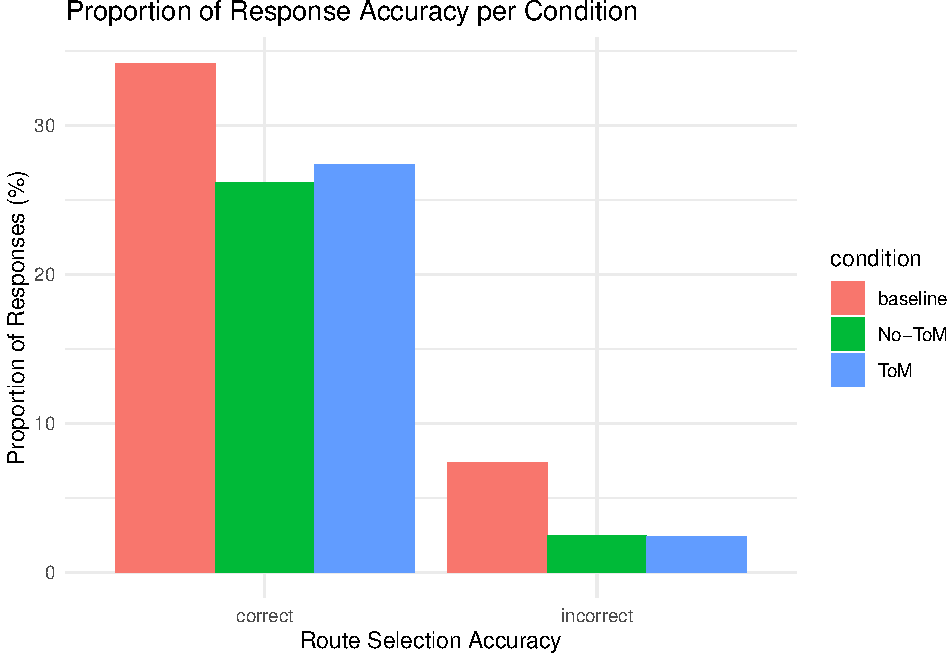
\includegraphics{T5_Data_wrangling_pdf_files/figure-latex/unnamed-chunk-22-1.pdf}

\hypertarget{wrap-up}{%
\section{Wrap up}\label{wrap-up}}

\begin{itemize}
\tightlist
\item
  Today we covered

  \begin{itemize}
  \tightlist
  \item
    How to wrangle and summarise numeric and categorical data
  \item
    Had brief explosure to checking the normality of numeric
    distributions
  \item
    You got your first taste of \texttt{ggplot2} plotting
  \end{itemize}
\item
  Next week there are no official lectures or tutorials. Please get in
  touch to discuss anything. I'm happy to help de-bug your code.
\end{itemize}

\hypertarget{cleanup}{%
\section{Cleanup}\label{cleanup}}

\begin{Shaded}
\begin{Highlighting}[]
\CommentTok{\# Clear data}
\FunctionTok{rm}\NormalTok{(}\AttributeTok{list =} \FunctionTok{ls}\NormalTok{())  }\CommentTok{\# Removes all objects from environment}

\CommentTok{\# Clear packages}
\FunctionTok{p\_unload}\NormalTok{(all)  }\CommentTok{\# Remove all contributed packages}

\CommentTok{\# Clear plots}
\FunctionTok{graphics.off}\NormalTok{()  }\CommentTok{\# Clears plots, closes all graphics devices}

\CommentTok{\# Clear console}
\FunctionTok{cat}\NormalTok{(}\StringTok{"}\SpecialCharTok{\textbackslash{}014}\StringTok{"}\NormalTok{)  }\CommentTok{\# Mimics ctrl+L}
\end{Highlighting}
\end{Shaded}

\hypertarget{references}{%
\section{References}\label{references}}

\end{document}
